\documentclass[10pt,a4paper]{article}
\usepackage[margin=2.1cm]{geometry}
\usepackage{amsmath,amssymb,bm}
\usepackage{booktabs,tabularx,array,multirow}
\usepackage{siunitx}
\usepackage{tikz}
\usetikzlibrary{arrows.meta,positioning,fit,calc,shapes.geometric}
\usepackage[hidelinks]{hyperref}
\usepackage{enumitem}
\usepackage{xcolor}
\usepackage{tcolorbox}
\usepackage{titlesec}
\usepackage{microtype}
\setlist{itemsep=1pt,topsep=3pt,leftmargin=1.4em}
\titlespacing*{\section}{0pt}{10pt}{4pt}
\titlespacing*{\subsection}{0pt}{7pt}{3pt}
\sisetup{per-mode=symbol}
\newcolumntype{L}{>{\raggedright\arraybackslash}X}
\definecolor{accent}{RGB}{31,78,121}
\newtcolorbox{keypt}{colback=accent!5,colframe=accent!60,boxrule=0.5pt,arc=1pt,left=4pt,right=4pt,top=2pt,bottom=2pt}
\newcommand{\R}{\mathbb{R}}
\newcommand{\T}{^{\!\top}}

\title{\textbf{ECM 2027 Simulation Track: Technical Primer}\\[2pt]
\large Physics, robotics, perception and learning behind the Chamber Service task}
\author{Team DIL-X}
\date{28 November 2026 \quad(starter code \texttt{rocochallenge/ecm2027\_sim\_track} @ \texttt{9759226})}

\begin{document}
\maketitle
\vspace{-6pt}
\begin{abstract}
\noindent This document explains, from first principles, every technical layer of the ECM 2027 simulation round: the software stack, the rigid-body and contact physics that PhysX integrates, the kinematics and control of the Galbot mobile manipulator, the camera model, the exact scoring physics of the six task stages, and the learning and planning methods that can produce a policy. All numerical parameters are taken from the released code (\texttt{galbot.py}, \texttt{assets\_cfg.py}, \texttt{galbot\_base\_velocity\_action.py}, \texttt{chamber\_service\_task.py}) and from organiser rulings on Discord up to 28 November 2026. Each section ends with what it implies for our design.
\end{abstract}

\tableofcontents
\newpage

%=====================================================================
\section{Problem statement}
%=====================================================================
A Galbot mobile manipulator stands in front of a table holding an industrial \emph{chamber} (a box with a hinged lid), a \emph{packing box}, a \emph{replacement box} and a \emph{sponge}. The robot must perform preventive maintenance in six sequential stages (Table~\ref{tab:stages}): open the lid, extract the old part, pack it, wipe the five inner faces of the cavity, install the replacement part, and close the lid. An episode lasts at most \SI{900}{\second} of simulated time; the score is 0--13.

Formally the task is a \textbf{partially observable Markov decision process} (POMDP) $\langle\mathcal S,\mathcal A,\mathcal O,P,Z,r\rangle$. The true state $s_t\in\mathcal S$ contains all body poses and velocities of the robot and the scene; the policy never sees it. At each control step ($\Delta t=\SI{20}{\milli\second}$) the policy receives an observation $o_t\sim Z(\cdot\mid s_t)$, namely three RGB images and proprioception, and returns an action $a_t\in\R^{19}$. The simulator advances $s_{t+1}\sim P(\cdot\mid s_t,a_t)$. The reward is the sparse, staged score. Our deliverable is a policy $\pi(a_t\mid o_{\le t})$ packaged as a Docker container.

\begin{figure}[h]
\centering
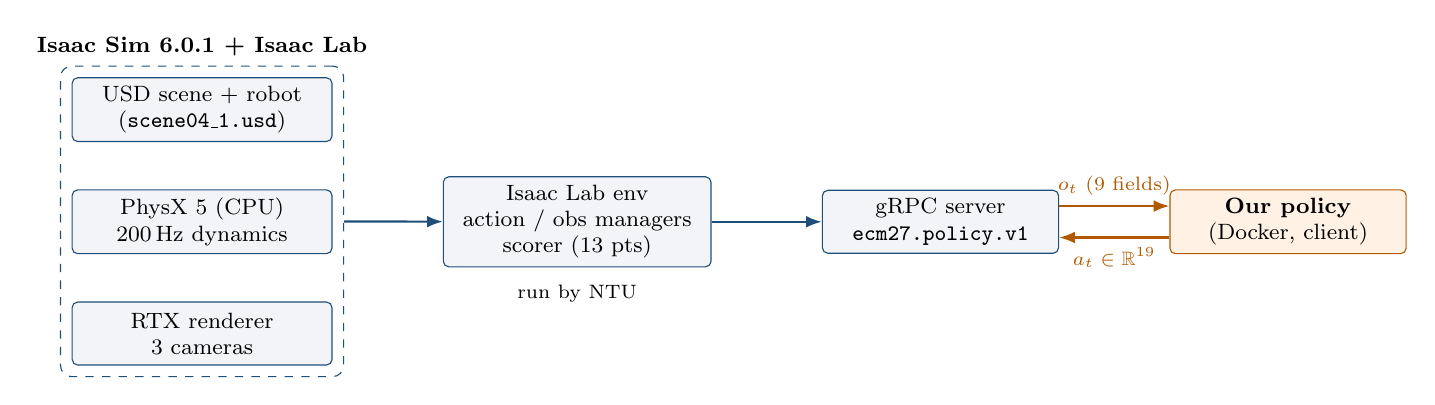
\begin{tikzpicture}[node distance=6mm and 9mm,
  box/.style={draw=accent,rounded corners=2pt,fill=accent!6,align=center,font=\footnotesize,minimum height=8mm,inner sep=3pt},
  arr/.style={-{Latex[length=2mm]},thick,accent}]
\node[box,minimum width=33mm] (usd) {USD scene + robot\\(\texttt{scene04\_1.usd})};
\node[box,below=of usd,minimum width=33mm] (physx) {PhysX 5 (CPU)\\\SI{200}{\hertz} dynamics};
\node[box,below=of physx,minimum width=33mm] (rtx) {RTX renderer\\3 cameras};
\node[draw=accent,dashed,rounded corners,fit=(usd)(physx)(rtx),inner sep=4pt,label={[font=\footnotesize\bfseries]above:Isaac Sim 6.0.1 + Isaac Lab}] (sim) {};
\node[box,right=14mm of physx,minimum width=34mm] (env) {Isaac Lab env\\action / obs managers\\scorer (13 pts)};
\node[box,right=14mm of env,minimum width=30mm] (srv) {gRPC server\\\texttt{ecm27.policy.v1}};
\node[box,right=14mm of srv,minimum width=30mm,fill=orange!10,draw=orange!70!black] (pol) {\textbf{Our policy}\\(Docker, client)};
\draw[arr] (sim) -- (env);
\draw[arr] (env) -- (srv);
\draw[arr,orange!70!black] ([yshift=2mm]srv.east) -- node[above,font=\scriptsize]{$o_t$ (9 fields)} ([yshift=2mm]pol.west);
\draw[arr,orange!70!black] ([yshift=-2mm]pol.west) -- node[below,font=\scriptsize]{$a_t\in\R^{19}$} ([yshift=-2mm]srv.east);
\node[font=\scriptsize,below=1mm of env,align=center] {run by NTU};
\end{tikzpicture}
\caption{Evaluation architecture. NTU runs the simulator; our container only runs a gRPC client that maps observations to actions at \SI{50}{\hertz}.}
\end{figure}

%=====================================================================
\section{Technology stack}
%=====================================================================
\begin{table}[h]\centering\footnotesize
\begin{tabularx}{\textwidth}{@{}p{3.1cm}L@{}}
\toprule
\textbf{Component} & \textbf{Role in the project}\\
\midrule
NVIDIA Isaac Sim 6.0.1 & Robotics simulator built on Omniverse Kit. Hosts the scene, steps physics (PhysX) and renders cameras (RTX ray tracing, which needs RT cores and so excludes A100/H100/V100 GPUs).\\
OpenUSD & Universal Scene Description: scene graph format for geometry, materials, physics properties (mass, friction, joints) and articulations. Assets live in \texttt{robofinals/data/assets/} (Git LFS).\\
NVIDIA PhysX 5 & Rigid-body and articulation dynamics with a contact solver. The evaluator uses the \textbf{CPU} pipeline (organiser ruling, 25 Nov).\\
Isaac Lab (rev \texttt{28a37ce}) + Isaac Lab Arena & Python RL/IL framework on top of Isaac Sim. Defines the \emph{manager-based environment}: action terms (DiffIK, binary gripper, base velocity), observation terms, events (randomised resets) and the task scorer.\\
PyTorch (CUDA 13.0 wheels) & Tensor backend of Isaac Lab, and our training framework.\\
gRPC + Protocol Buffers & Remote-procedure-call protocol between evaluator (server) and policy (client): \texttt{GetObservation}, \texttt{Step}. Messages carry raw image bytes and float32 vectors.\\
Docker & Packaging of the policy (Linux amd64 image). Submitted via a private Hugging Face repository, with access granted to \texttt{sgeaichallenge}.\\
HDF5 (\texttt{h5py}) & Format of the demonstration data (\texttt{galbot\_success.hdf5}, about \SI{2.9}{\giga\byte} per episode): actions, states, camera arrays. LeRobot copies are deprecated.\\
Hugging Face Hub & Distribution of the dataset (\texttt{rocochallenge2025/ecm2027\_sim\_data}, about \SI{1.55}{\tera\byte}) and of our submission.\\
Learning libraries & Behaviour cloning / ACT / Diffusion Policy (Section~\ref{sec:learning}); vision backbones (ResNet, ViT, DINOv2) with public pretrained weights (allowed).\\
\bottomrule
\end{tabularx}
\caption{Technology stack.}
\end{table}

%=====================================================================
\section{Simulation physics}
%=====================================================================
\subsection{Time discretisation}
The Galbot environment overrides the defaults to a physics step $h=\SI{5}{\milli\second}$ (\SI{200}{\hertz}) with decimation 4. Each policy action is therefore held constant (zero-order hold) for four physics sub-steps, giving a control period $\Delta t=4h=\SI{20}{\milli\second}$ (\SI{50}{\hertz}). One episode of \SI{900}{\second} is $45\,000$ control steps. Sensors run at their own rates: the head camera updates at \SI{30}{\hertz} and the wrist cameras at \SI{20}{\hertz}. Consecutive observations can therefore contain \emph{identical images}, and image-conditioned policies should not assume a fresh frame every step.

\subsection{Rigid-body and articulation dynamics}
Every free body obeys the Newton--Euler equations
\begin{equation}
m\dot{\bm v}=\bm f_{\text{ext}}+m\bm g,\qquad \bm I\dot{\bm\omega}+\bm\omega\times\bm I\bm\omega=\bm\tau_{\text{ext}} .
\end{equation}
The robot is an \emph{articulation}: a tree of links joined by revolute or prismatic joints, simulated in reduced (joint) coordinates $\bm q$ with Featherstone-type algorithms. Its equation of motion is
\begin{equation}
\bm M(\bm q)\ddot{\bm q}+\bm C(\bm q,\dot{\bm q})\dot{\bm q}+\bm g(\bm q)=\bm\tau_{\text{drive}}+\bm J_c\T(\bm q)\,\bm f_c ,
\label{eq:eom}
\end{equation}
with mass matrix $\bm M$, Coriolis/centrifugal terms $\bm C$, gravity torque $\bm g$, joint drive torques $\bm\tau_{\text{drive}}$, and contact forces $\bm f_c$ mapped through the contact Jacobian $\bm J_c$. The Galbot articulation has \textbf{77 joints} (the length of \texttt{joint\_pos}). These cover the legs/torso, head, two 7-DoF arms, two grippers (each 1 driven plus 5 mimic joints), and 4 omni wheels with their rollers.

\subsection{Contact and friction}
PhysX resolves contacts as constraints with an iterative solver (TGS in Isaac Lab). For each contact point with normal force $f_n\ge 0$ and tangential force $\bm f_t$ it enforces non-penetration and the \textbf{Coulomb friction cone}
\begin{equation}
\|\bm f_t\|\le\mu f_n .
\end{equation}
Relevant solver settings from the code are listed below.
\begin{itemize}
\item \textbf{Position/velocity iterations 48/8} for the robot and the sponge, raised from 24/4. More position iterations reduce finger--part interpenetration under grasp; more velocity iterations tighten the friction hold.
\item \textbf{Max depenetration velocity \SI{4}{\metre\per\second}.} This is how fast overlapping bodies are pushed apart. Higher values ``fling'' thin parts (the comment in the code notes that 5 did).
\item \textbf{Sleep and stabilisation thresholds.} Near-static bodies are frozen to save computation. Combined with the scorer's ``still for \SI{1}{\second}'' conditions, this means a gently released object settles quickly, while a dropped one bounces and resets the timer.
\item Gripper fingers have \emph{filtered collision pairs} with each other, so they can close fully while still colliding with objects.
\end{itemize}
\begin{keypt}\footnotesize\textbf{Why CPU physics matters.} The parallel GPU solver orders constraint updates differently and is non-deterministic, so the same action sequence can diverge (organisers saw demo replays ``sway'' on GPU physics). The evaluator uses CPU physics, so we must collect data, replay and test on CPU physics too.\end{keypt}

\subsection{Joint drives: implicit PD actuators}
All robot joints use \emph{implicit} PD drives, which PhysX integrates inside the solver and which are therefore stable at high gains:
\begin{equation}
\tau=\operatorname{clip}\!\big(k_p(q^\ast-q)+k_d(\dot q^\ast-\dot q),\;-\tau_{\max},\tau_{\max}\big).
\end{equation}
Treating one joint as a second-order system with effective inertia $I$ gives natural frequency $\omega_n=\sqrt{k_p/I}$ and damping ratio $\zeta=k_d/(2\sqrt{k_pI})$.

\begin{table}[h]\centering\footnotesize
\begin{tabular}{@{}lrrrrl@{}}
\toprule
Group & $k_p$ & $k_d$ & $\tau_{\max}$ & $\dot q_{\max}$ & Note\\
\midrule
Arms (2$\times$7) & 1400 & 320 & 1200 & \SI{1.5}{\radian\per\second} & stiff: holds pose against grasp wrenches\\
Grippers & 69 & 1.17 & \SI{6}{\newton\metre} & 6.1 & armature $5\times10^{-3}$; open $0$, closed $\SI{1.703}{\radian}$\\
Legs (mobile) & $10^5$ & $10^4$ & 1000 & 1.0 & effectively locked stand pose\\
Head & 80 & 10 & 4 & 1.5 & not commanded by the policy\\
Wheels & 50\,000 & 1000 & 40 & 1.0 & velocity targets (visual only, see \S\ref{sec:base})\\
\bottomrule
\end{tabular}
\caption{Actuator parameters (\texttt{assets\_cfg.py}).}
\end{table}

\noindent\textbf{Worked example: the gripper.} The code's design comment assumes a part of mass $m=\SI{1.5}{\kilo\gram}$ and friction $\mu=0.4$. To hold the part against gravity with two opposing fingers, friction must supply $mg$, so each finger needs a normal force $f_n\ge mg/(2\mu)=\SI{18.4}{\newton}$. With a finger lever arm $r=\SI{0.05}{\metre}$ and 6 coupled joints, the required drive torque is $6\cdot f_n r\approx\SI{5.5}{\newton\metre}$, hence $\tau_{\max}=6$. With $I\approx$ armature $=5\times10^{-3}$: $\omega_n=\sqrt{69/0.005}\approx\SI{117}{\radian\per\second}$ and $\zeta=1.17/(2\sqrt{69\cdot0.005})\approx1.0$, i.e.\ \textbf{critically damped}. The gripper is a \emph{binary} action: a command below 0 closes it (target \SI{1.703}{\radian}), and a command of 0 or more opens it. Grip force is therefore not controllable; heavy or slippery objects must be grasped near their centre of mass to limit the torque about the contact axis.

\subsection{The mobile base}\label{sec:base}
The base is \emph{not} driven by wheel--ground friction. At every control step the base action writes the root velocity directly into the simulator, rotating the body-frame command into the world frame:
\begin{equation}
\bm v_W=\bm R_{WB}\begin{bmatrix}v_x\\v_y\\0\end{bmatrix},\qquad \omega_{z,W}=\omega_z .
\end{equation}
The base is therefore \textbf{holonomic}: it can translate in any direction and rotate independently. The four omni-wheel joint velocity targets are only set for visual consistency, through the mixing matrix $\bm W$ (scaled by 0.01):
\begin{equation}
\bm w=\bm W\begin{bmatrix}v_x\\v_y\\\omega_z\end{bmatrix},\quad
\bm W=\begin{bmatrix}1&-1&-1\\1&1&1\\1&1&-1\\1&-1&1\end{bmatrix},\quad
\bm W\T\bm W=4\bm I_3\;\Rightarrow\;\bm W^{+}=\tfrac14\bm W\T .
\end{equation}
Because the columns of $\bm W$ are orthogonal, the least-squares inverse is simply $\tfrac14\bm W\T$. This is exactly the formula that converts the dataset's legacy 4-wheel actions to $(v_x,v_y,\omega_z)$.

\textbf{Command smoothing.} Native 19-D base commands pass through an exponential moving average (EMA):
\begin{equation}
\bm u_k=\bm u_{k-1}+\alpha(\bm r_k-\bm u_{k-1}),\qquad\alpha=0.1 .
\end{equation}
This is a first-order low-pass filter with time constant $\tau=-\Delta t/\ln(1-\alpha)\approx\SI{0.19}{\second}$, so a step command reaches 95\,\% after about 28 steps (\SI{0.57}{\second}). Legacy 20-D actions bypass the filter, because they were recorded after teleop smoothing. A base controller must account for this lag, or it will overshoot.

%=====================================================================
\section{Robot kinematics}
%=====================================================================
\subsection{Coordinate frames}
\begin{figure}[h]\centering
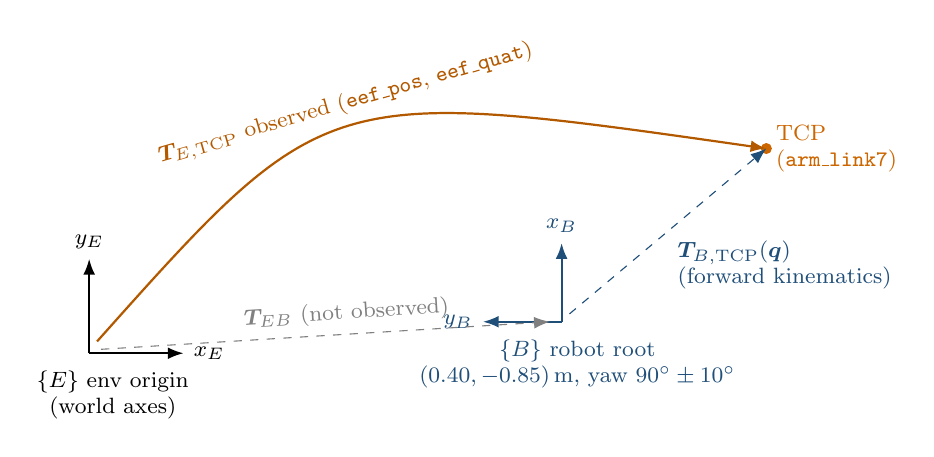
\begin{tikzpicture}[font=\footnotesize,>={Latex[length=2mm]}]
% env frame
\draw[->,thick] (0,0) -- (1.2,0) node[right]{$x_E$};
\draw[->,thick] (0,0) -- (0,1.2) node[above]{$y_E$};
\node[below,align=center] at (0.3,-0.1) {$\{E\}$ env origin\\(world axes)};
% base frame (yaw 90 deg)
\coordinate (B) at (6,0.4);
\draw[->,thick,accent] (B) -- ++(0,1.0) node[above]{$x_B$};
\draw[->,thick,accent] (B) -- ++(-1.0,0) node[left]{$y_B$};
\node[accent,below,align=center] at (6.2,0.3) {$\{B\}$ robot root\\$(0.40,-0.85)$\,m, yaw $90^\circ\pm10^\circ$};
% TCP
\coordinate (P) at (8.6,2.6);
\fill[orange!80!black] (P) circle (2pt) node[right,align=left]{TCP\\(\texttt{arm\_link7})};
% transforms
\draw[->,dashed,gray] (0.15,0.05) -- node[above,sloped,pos=0.55]{$\bm T_{EB}$ (not observed)} ($(B)+(-0.15,0)$);
\draw[->,dashed,accent] ($(B)+(0.1,0.1)$) -- node[below right,align=left]{$\bm T_{B,\mathrm{TCP}}(\bm q)$\\(forward kinematics)} (P);
\draw[->,orange!70!black,thick] (0.1,0.15) .. controls (3,3.4) .. node[above,sloped]{$\bm T_{E,\mathrm{TCP}}$ observed (\texttt{eef\_pos}, \texttt{eef\_quat})} (P);
\end{tikzpicture}
\caption{Frames. Observations give the tool pose in $\{E\}$; arm actions are tool poses in $\{B\}$.}
\end{figure}
Rigid transforms are elements of $SE(3)$, written as $\bm T=\begin{bmatrix}\bm R&\bm t\\\bm 0&1\end{bmatrix}$, and compose as $\bm T_{AC}=\bm T_{AB}\bm T_{BC}$. The interface mixes frames:
\begin{itemize}
\item \textbf{Observation} \texttt{eef\_pos}, \texttt{eef\_quat}: the tool pose $\bm T_{E,\mathrm{TCP}}$, expressed in world axes relative to the environment origin (confirmed 21--25 Nov).
\item \textbf{Action} \texttt{[0:7]}, \texttt{[7:14]}: the desired tool pose $\bm T^\ast_{B,\mathrm{TCP}}$ in the robot root frame $\{B\}$, which Isaac Lab's DiffIK action term expects.
\end{itemize}
Converting a world-frame target into an action needs the base pose: $\bm T^\ast_{B,\mathrm{TCP}}=\bm T_{EB}^{-1}\bm T^\ast_{E,\mathrm{TCP}}$.

\begin{keypt}\footnotesize\textbf{Free localisation from proprioception.} $\bm T_{EB}$ is not observed directly, but it can be recovered exactly. Forward kinematics of the arm joints (in \texttt{joint\_pos}) gives $\bm T_{B,\mathrm{TCP}}(\bm q)$, and the observation gives $\bm T_{E,\mathrm{TCP}}$, so
$\bm T_{EB}=\bm T_{E,\mathrm{TCP}}\,\bm T_{B,\mathrm{TCP}}(\bm q)^{-1}.$
Two arms give two independent estimates. This yields the robot's pose in the scene, which is permitted input (organisers, 23 Nov), and it is what lets us undo the $\pm\SI{10}{\centi\metre}/\pm10^\circ$ start randomisation.\end{keypt}

\subsection{Rotations and quaternions}
Orientations use unit quaternions $\bm q=(x,y,z,w)$ (scalar last, Hamilton convention). A rotation by angle $\theta$ about unit axis $\hat{\bm n}$ is $\bm q=(\hat{\bm n}\sin\tfrac\theta2,\cos\tfrac\theta2)$. Composition is the Hamilton product $\bm q_1\otimes\bm q_2$ (apply $\bm q_2$ first), and the inverse of a unit quaternion is its conjugate. Two practical pitfalls:
\begin{itemize}
\item \textbf{Double cover.} $\bm q$ and $-\bm q$ are the same rotation. Learned policies must canonicalise the sign (e.g.\ force $w\ge0$) or regress a continuous representation (the 6-D rotation representation), or the loss sees jumps.
\item \textbf{Normalisation.} The evaluator rejects actions whose quaternion norm is below $10^{-6}$. Interpolate orientations with \emph{slerp}, $\bm q(s)=\bm q_0\otimes(\bm q_0^{-1}\otimes\bm q_1)^s$, not with a linear blend.
\end{itemize}

\subsection{Forward kinematics and the Jacobian}
Each 7-DoF arm is a serial chain. Forward kinematics (FK) is a product of joint transforms, $\bm T_{B,\mathrm{TCP}}(\bm q)=\prod_{i=1}^{7}\bm T_{i-1,i}(q_i)$. The geometric Jacobian $\bm J(\bm q)\in\R^{6\times7}$ maps joint velocities to the tool's spatial velocity: $[\dot{\bm p};\bm\omega]=\bm J\dot{\bm q}$. With 7 joints for a 6-D task, each arm is \textbf{kinematically redundant}: there is a one-dimensional null space (elbow ``self-motion''), which allows obstacle avoidance, for example keeping the elbow away from the lid.

\subsection{Differential inverse kinematics (DLS)}
The action does not specify joint angles; Isaac Lab converts the pose target into joint targets every control step with \textbf{damped least squares} (DLS) differential IK:
\begin{equation}
\Delta\bm q=\bm J\T\left(\bm J\bm J\T+\lambda^2\bm I_6\right)^{-1}\bm e,\qquad
\bm e=\begin{bmatrix}\bm p^\ast-\bm p\\ \bm\phi(\bm q^\ast\otimes\bm q^{-1})\end{bmatrix},
\label{eq:dls}
\end{equation}
where $\bm\phi(\cdot)$ is the axis--angle vector of the orientation error and $\lambda$ is the damping (Isaac Lab default $0.01$). The joint target $\bm q+\Delta\bm q$ is then tracked by the PD drives. The properties that matter for us:
\begin{itemize}
\item \textbf{Singularities.} When $\bm J$ loses rank (arm fully stretched, wrist axes aligned), plain pseudo-inverse IK explodes. DLS trades accuracy for bounded joint steps; near singularities the tool lags its target.
\item \textbf{One linearised step per tick.} Equation~\eqref{eq:dls} is a first-order step, not a full solve. Far-away targets produce large, curved, poorly predictable motions, possibly colliding on the way. Feed \emph{nearby} waypoints along an interpolated path.
\item \textbf{Joint limits and speed.} With $\dot q_{\max}=\SI{1.5}{\radian\per\second}$ and $\Delta t=\SI{20}{\milli\second}$, each joint moves at most \SI{0.03}{\radian} per step. Commanding faster motion only increases tracking error.
\item \textbf{Reachability.} The arm length is about \SI{0.7}{\metre}. The base must be positioned so that each sub-task lies within the dexterous workspace, which matters especially for the far cavity wall during wiping.
\end{itemize}

\subsection{Trajectory generation}
Between waypoints, a \textbf{minimum-jerk} time scaling gives smooth, contact-friendly motion: $\bm p(t)=\bm p_0+(\bm p_1-\bm p_0)\,s(\tau)$ with $s(\tau)=10\tau^3-15\tau^4+6\tau^5$ and $\tau=t/T$, combined with slerp for orientation. This profile has zero velocity and acceleration at both ends, which helps the ``still for \SI{1}{\second}'' scoring conditions.

%=====================================================================
\section{Perception}
%=====================================================================
\subsection{Sensors}
\begin{table}[h]\centering\footnotesize
\begin{tabular}{@{}llll@{}}
\toprule
Camera & Mount & Output & Rate\\
\midrule
Head (\texttt{first\_person\_camera\_rgb}) & head link, fixed offset & $480\times640\times3$ RGB, pinhole, clip 0.1--\SI{15}{\metre} & \SI{30}{\hertz}\\
Left / right wrist & on each hand link & $224\times224\times3$ RGB, clip 0.03--\SI{10}{\metre} & \SI{20}{\hertz}\\
\bottomrule
\end{tabular}
\caption{Cameras. RGB only: there is \emph{no depth} and \emph{no force/torque sensing}.}
\end{table}
\noindent Each camera is a pinhole: a 3-D point $\bm X_C$ in camera coordinates projects to pixel $\tilde{\bm u}=\bm K\bm X_C/Z_C$ with intrinsics $\bm K=\begin{bmatrix}f_x&0&c_x\\0&f_y&c_y\\0&0&1\end{bmatrix}$. Camera extrinsics follow from the mount offsets in \texttt{galbot.py} and FK. The full chain $\bm T_{E,C}=\bm T_{EB}\,\bm T_{B,\text{link}}(\bm q)\,\bm T_{\text{link},C}$ is therefore known at every step, so a pixel detection can be turned into a 3-D ray in the scene.

\subsection{Object pose estimation}
The organisers forbid simulator object poses at runtime, and since the official runs shift the boxes and chamber slightly, objects must be localised from RGB. Options:
\begin{itemize}
\item \textbf{Known geometry + PnP.} The CAD dimensions of the chamber, boxes and part are allowed priors. Detect $n$ 2-D keypoints (corners, hinge, handle) with a CNN, then solve Perspective-$n$-Point, $\min_{\bm R,\bm t}\sum_i\|\bm u_i-\pi(\bm K(\bm R\bm X_i+\bm t))\|^2$, for the 6-D pose.
\item \textbf{Multi-view triangulation.} The same feature seen by the head camera and a wrist camera (or by one wrist camera at two arm poses) gives depth by intersecting rays. The baseline is known from FK.
\item \textbf{Direct regression.} A network predicts an object's position relative to the robot from the images and proprioception. It is trained on labels taken offline from simulator state, which is explicitly allowed for training.
\item \textbf{Visual servoing / implicit.} An end-to-end policy (Section~\ref{sec:learning}) never estimates poses explicitly and learns the image-to-action map instead. This is less interpretable and needs more data.
\end{itemize}
\textbf{Domain shift.} The 27 Nov release added a scene with a background and full textures. Until it is confirmed which scene the evaluator renders, perception must be robust to both. Use re-rendered data from both scenes and colour, lighting and crop augmentation.

%=====================================================================
\section{The task and its scoring physics}
%=====================================================================
The scorer (\texttt{chamber\_service\_task.py}) evaluates stages strictly in order: a stage is only assessed once every point of the previous stage is credited. All thresholds are in SI units.

\begin{table}[h]\centering\footnotesize
\begin{tabularx}{\textwidth}{@{}clcL@{}}
\toprule
\# & Stage & Pts & Exact success condition\\
\midrule
1 & Open lid & 2 & (a) front edge raised $\ge\SI{1}{\centi\metre}$: $L\sin\theta\ge0.01$, $L=\SI{0.698}{\metre}$, i.e.\ $\theta\ge0.82^\circ$; (b) normalised opening $\ge0.4$ \emph{and} $|\dot\theta|\le\SI{0.1}{\radian\per\second}$ held for \SI{1}{\second}.\\
2 & Extract old part & 1 & Part centre lifted $\ge\SI{1}{\centi\metre}$ above its resting height (latched \SI{0.5}{\second} after reset).\\
3 & Pack into box & 1 & Part centre inside the box footprint ($\pm\SI{0.175}{\metre}$), below the rim, speed $\le\SI{0.05}{\metre\per\second}$ for \SI{1}{\second}.\\
4 & Wipe cavity & 6 & (a) sponge lifted $\ge\SI{1}{\centi\metre}$; (b) per face (4 walls + floor, any order): sponge--chamber contact while the sponge centre is inside the cavity, nearest face within \SI{0.08}{\metre}, \emph{continuous} for \SI{0.5}{\second}.\\
5 & Place replacement & 2 & (a) new part lifted $\ge\SI{1}{\centi\metre}$; (b) centre within \SI{5}{\centi\metre} of the old part's latched pose, speed $\le\SI{0.05}{\metre\per\second}$, for \SI{1}{\second}.\\
6 & Close lid & 1 & Normalised opening $\le0.005$ and $|\dot\theta|\le\SI{0.1}{\radian\per\second}$ for \SI{1}{\second}.\\
\bottomrule
\end{tabularx}
\caption{Stages and thresholds. The sponge should be returned to the table after wiping (no points). The inner cavity is $0.688\times0.694\times\SI{0.30}{\metre}$.}
\label{tab:stages}
\end{table}

\subsection{Physics of each stage}
\textbf{Lid (hinge mechanics).} The lid rotates about its rear hinge. To lift it, the applied force must overcome the gravity torque $\tau_g=m_\ell g\frac L2\cos\theta$, which is largest when the lid is nearly closed. A force $F$ applied at distance $r$ from the hinge, perpendicular to the lid, gives $\tau=rF$. Pushing at the front edge ($r=L$) needs the least force, and the end-effector path must follow the arc $\bm p(\theta)=\bm p_h+L(\cos\theta\,\hat{\bm x}+\sin\theta\,\hat{\bm z})$ about the hinge. A straight-line pull fights the constraint and slips. ``Stable open'' requires leaving the lid past 40\,\% of its range and releasing without it falling back, so it should be pushed beyond the balance point.

\textbf{Pick and place (friction grasp).} The grasp holds by friction alone (Section~3.4). Lift slowly, because inertial loads add $m\,\ddot z$ to the required friction force. When placing, lower to just above the surface and open the gripper: a drop larger than a few millimetres can bounce and break the \SI{0.05}{\metre\per\second} stillness condition. Placing the replacement needs a \SI{5}{\centi\metre} accuracy relative to where the \emph{old} part rested, so remember that pose (in $\{E\}$) when extracting it.

\textbf{Wiping (contact without force sensing).} There is no force sensor, but contact force can be produced through the stiffness of position control. If the commanded tool position is offset by $\bm\delta$ into the wall, the arm's PD drives act like a Cartesian spring with stiffness $\bm K_x\approx\bm J^{-\top}\bm K_q\bm J^{-1}$ (with $\bm K_q=\operatorname{diag}(k_p)$), so the normal force is $\bm f\approx\bm K_x\bm\delta$. With $k_p=1400$ the effective stiffness is very high: a few millimetres of offset already gives large forces, risking penetration, jitter or the sponge slipping out of the grasp. Use small offsets and keep the sponge face parallel to the wall. Each face needs \SI{0.5}{\second} of \emph{uninterrupted} contact (the timer resets to zero on loss of contact), and the sponge centre must stay inside the cavity within \SI{8}{\centi\metre} of that face. A slow stroke ($\sim$\SI{1}{\second}) pressed against each wall and the floor is enough; covering the whole area is not required. This stage is worth 6 of the 13 points.

\textbf{Closing.} This is the opening motion in reverse, but gravity now helps. Lower the lid under control rather than letting it slam, since a bounce delays the \SI{1}{\second} stillness timer.

%=====================================================================
\section{Policy design: planning, control and learning}\label{sec:learning}
%=====================================================================
\subsection{Expected score and why reliability dominates}
Because stages unlock in sequence, if stage $i$ succeeds with probability $p_i$ (given the previous stages succeeded) and is worth $c_i$ points, then approximately
\begin{equation}
\mathbb E[\text{score}]=\sum_{k=1}^{6}c_k\prod_{i=1}^{k}p_i .
\end{equation}
For example, $p=(0.9,0.9,0.9,0.8,0.7,0.9)$ with $c=(2,1,1,6,2,1)$ gives $1.8+0.81+0.73+3.50+0.82+0.37\approx8.0/13$. Improving stage 1 from 0.9 to 0.99 raises every later term, so early-stage robustness has the largest marginal value. The final score is the mean over 20 episodes, with standard error $\sigma/\sqrt{20}$. Local evaluation needs a comparable number of randomised episodes before we can trust a difference between two policies.

\subsection{Approach A: hierarchical stage machine}
A finite-state machine sequences skills: \textsc{Navigate} $\rightarrow$ \textsc{OpenLid} $\rightarrow$ \textsc{Extract} $\rightarrow$ \textsc{Pack} $\rightarrow$ \textsc{Wipe}$\times5$ $\rightarrow$ \textsc{ReturnSponge} $\rightarrow$ \textsc{Place} $\rightarrow$ \textsc{CloseLid}. Each skill:
\begin{enumerate}
\item estimates the relevant object pose from perception (Section~5) and the base pose from FK (Section~4.1);
\item replays key-poses taken from the demonstrations \emph{relative to the object} ($\bm T_{\text{obj},\mathrm{TCP}}$), which transfers them to the randomised layout;
\item interpolates them with minimum-jerk and slerp, converts to $\{B\}$ and streams them as actions;
\item checks completion from observations (gripper closure in \texttt{gripper\_pos}, tool height), with timeouts and retries.
\end{enumerate}
The base is driven to a pre-recorded work pose with a proportional controller on the pose error expressed in $\{B\}$, saturated and lag-compensated for the EMA filter. Hybrid scripted and learned control is explicitly allowed (organisers, 25 Nov).

\subsection{Approach B: imitation learning}
\textbf{Behaviour cloning} fits $\pi_\theta$ to demonstration pairs $(o_t,a_t)$ by supervised regression, $\min_\theta\mathbb E\,\ell(\pi_\theta(o_t),a_t)$. Its main failure mode is \emph{covariate shift}: small errors take the robot to states absent from the data, and errors compound over a horizon $T$ (worst case $O(T^2\epsilon)$; Ross et al.). Three remedies matter here:
\begin{itemize}
\item \textbf{Action chunking (ACT).} A transformer, trained as a conditional VAE, predicts the next $k$ actions at once and blends overlapping chunks by temporal ensembling. This shortens the effective horizon by a factor of $k$ and handles pauses in the demonstrations.
\item \textbf{Diffusion Policy.} This represents $p(a_{t:t+k}\mid o_t)$ by a denoising diffusion model trained with $\mathbb E\|\bm\epsilon-\bm\epsilon_\theta(\bm a^{(n)},n,o_t)\|^2$. It captures \emph{multimodal} demonstrations (e.g.\ wiping left-to-right or right-to-left) that a mean-squared-error regressor would average into an invalid motion.
\item \textbf{Data processing.} Convert 20-D actions to 19-D (with $\bm W^+$), canonicalise quaternions, normalise per dimension, align the 30/\SI{20}{\hertz} images to the \SI{50}{\hertz} actions, re-render images for batch 2, and use CPU-physics replays to verify each conversion. Note the observation includes the previous action, which can cause a ``copycat'' shortcut where the policy just repeats it; consider dropping it from the inputs.
\end{itemize}

\subsection{Approach C: hybrid (recommended)}
Use the stage machine for navigation, sequencing and the precise geometric steps (lid arc, placement), and learned components where geometry is hard to script: the perception models, and possibly a learned wiping or grasping skill. This keeps failures diagnosable per stage, which matters with only five scored submissions and 5 working days of feedback latency.

%=====================================================================
\section{Systems engineering}
%=====================================================================
\begin{itemize}
\item \textbf{Interface.} Batched: $N$ environments (1--27) per call, with per-environment reset of internal state when \texttt{terminated} or \texttt{truncated} is set. \texttt{INVALID\_ARGUMENT} is returned for a wrong dimension, NaN or Inf values, a quaternion norm below $10^{-6}$, or positions beyond \SI{\pm10}{\metre}. \texttt{FAILED\_PRECONDITION} signals a wall-clock reset: call \texttt{GetObservation} again.
\item \textbf{Timing budget.} \SI{900}{\second} of simulated time is $45\,000$ steps within a \SI{300}{\minute} wall-clock limit, so the full loop (rendering, physics, gRPC and inference) must sustain at least 2.5 steps per second, and much more in practice. Keep model inference well under \SI{100}{\milli\second}, or run the heavy model at a lower rate and hold or interpolate its outputs.
\item \textbf{Determinism and testing.} Use CPU physics locally. Our mock server (\texttt{team/tools/mock\_eval\_server.py}) tests the protocol without Isaac Sim, and the real evaluator (\texttt{run\_eval\_env.sh}) with randomised resets gives the score.
\item \textbf{Submission strategy.} At most 5 valid submissions, and the \emph{last} one is the final score. Never submit a policy that is worse in local evaluation than the previous one.
\end{itemize}

%=====================================================================
\section*{Further reading}
\begin{small}
\begin{enumerate}[label={[\arabic*]},leftmargin=2em]
\item M.~Mittal et al., ``Orbit: A unified simulation framework for interactive robot learning environments,'' \emph{IEEE RA-L}, 2023 (Isaac Lab).
\item R.~Featherstone, \emph{Rigid Body Dynamics Algorithms}. Springer, 2008.
\item B.~Siciliano, L.~Sciavicco, L.~Villani, G.~Oriolo, \emph{Robotics: Modelling, Planning and Control}. Springer, 2009.
\item S.~R.~Buss, ``Introduction to inverse kinematics with Jacobian transpose, pseudoinverse and damped least squares methods,'' 2004.
\item K.~M.~Lynch, F.~C.~Park, \emph{Modern Robotics: Mechanics, Planning, and Control}. Cambridge Univ. Press, 2017.
\item T.~Flash, N.~Hogan, ``The coordination of arm movements: an experimentally confirmed mathematical model,'' \emph{J. Neurosci.}, 1985.
\item S.~Ross, G.~Gordon, D.~Bagnell, ``A reduction of imitation learning and structured prediction to no-regret online learning,'' \emph{AISTATS}, 2011.
\item T.~Z.~Zhao, V.~Kumar, S.~Levine, C.~Finn, ``Learning fine-grained bimanual manipulation with low-cost hardware'' (ACT), \emph{RSS}, 2023.
\item C.~Chi et al., ``Diffusion Policy: Visuomotor policy learning via action diffusion,'' \emph{RSS}, 2023.
\item Y.~Zhou et al., ``On the continuity of rotation representations in neural networks,'' \emph{CVPR}, 2019.
\end{enumerate}
\end{small}
\end{document}
